\chapter{Xây dựng hệ thống phân loại tự động}
\paragraph{Giới thiệu} Qua các chương trước, chúng em đã trình bày các cơ sở lý thuyết gồm OWL 2, SWRL, đề ra các thiết kế cho hệ thống và thiết kế một ontology sử dụng cho việc phân loại. Trong chương này, chúng em sẽ trình bày lại quá trình xây dựng hệ thống phân loại dựa trên các thiết kế ở chương trước.
\section{UI của ứng dụng - OWLEditorUI}
\subsection{Giới thiệu OWLEditorUI}
Lớp này được mở rộng từ lớp \textbf{UI} của Vaadin - chức năng cơ bản của \textbf{UI} là nơi khởi tạo mọi thành phần giao diện và trình bày nó dưới dạng HTML trên web page, OWLEditorUI mở rộng các chức năng trên như sau:
\begin{itemize}
\item Chứa EntryView, MainView (các View này chứa tất cả thành phần giao diện của hệ thống)
\item Cập nhật và cài đặt MainView khi ontology được nạp vào EntryView.
\item Cập nhật trạng thái khi người dùng refresh trang.
\item Nạp (inject) OWLEditorKit và cung cấp nó qua phương thức tĩnh (static).
\item Nạp EventBus và cung cấp qua các phương thức tĩnh.
\item Nạp HttpSession và cung cấp qua phương thức tĩnh .
\end{itemize}
\subsection{Chi tiết các chức năng của OWLEditorUI}
Trước khi đi vào chi tiết các chức năng trên, chúng em muốn giới thiệu sơ quan về việc cách Spring Boot \cite{springboot} hoạt động, các Annotation đáng chú ý được sử dụng trong việc xây dựng hệ thống.
\\
\textbf{Spring Boot} Khi chương trình khởi động - ở đây không nói đến khi chúng ta nhập URL vào webpage mà chúng em đang muốn nói đến khi chương trình được nạp vào một hệ thống Servlet như Tomcat, Jetty thì điểm đầu tiên của nó xuất phát sẽ từ đối tượng sau:
\begin{verbatim}
@SpringBootApplication public class OWLEditorApplication {
    public static void main(String[] args) {
       SpringApplication.run(OWLEditorApplication.class, args); }
}
\end{verbatim} 
@SpringBootApplication là một tên thay thế cho 3 annotation gồm \textbf{@Configuration}, \textbf{@EnableAutoConfiguration} và \textbf{@ComponentScan} (sẽ được giới thiệu ở dưới), mục tiêu của đối tượng này là khởi động ứng dụng, quét hết trong package hiện hành tới package con để tìm các Component Bean cần thiết để khởi tạo và thực thi các Bean đó. Cụ thể ở đây, nó sẽ quét vào tìm thấy \textbf{OWLEditorUI} được đánh dấu bằng \textbf{@VaadinUI} và chạy theo cấu hình có săn được định nghĩa trong theo dự án Spring 4 Vaadin \cite{spring4vaadin}. Từ đây mọi thứ sẽ diễn ra trong \textbf{OWLEditorUI}. Ý nghĩa của các Annotation:
\begin{itemize}	
\item \textbf{@VaadinUI} Là annotation của dự án Spring 4 Vaadin \cite{spring4vaadin} khai báo một lớp là một Bean và là một Vaadin \textbf{UI} cho hệ thống Spring Boot.
\item \textbf{@VaadinComponent} Là annotation của dự án Spring 4 Vaadin, tương tự annotation @Component của Spring Framework: khai báo đây là một Bean cơ bản nhất cho hệ thống Spring Boot.
\item \textbf{@Repository} Là annotation của Spring Framework, khai báo một đối tượng là một Bean với tính chất là một nơi để lấy và khai thác dữ liệu, OWLEditorKit được khai báo bằng annotation này.
\item \textbf{@Autowired} Là annotaion của Spring Framework, dùng nạp tự động các Bean đã được khai báo (bằng các annotatio như @VaadinComponent, @Component, @Repository, ...) vào hệ thống, cụ thể chúng em dùng chúng để nạp OWLEditorKit, HttpSession và OWLEditorEventBus vào OWLEditorUI.
\item \textbf{@Theme} Là annotation của Vaadin dùng để nạp thành phần tùy chỉnh CSS cho toàn bộ giao diện của hệ thống.
\item \textbf{@EnableAutoConfiguration} Là annotation của Spring Boot, bật tính năng cấu hình tự động (mọi cấu hình về DataBase, Base Url,... sẽ ở trạng thái mặc định).
\item \textbf{@ComponentScan} Là annotation của Spring, tự động quét và tìm các Bean từ package hiện hành và khởi tạo chúng.
\item \textbf{@Nonnull} Là annotation từ JSR-305, đảm bảo tham số nhập vào không được null, nếu null tự động throw NullPointerException.
\end{itemize}
\subsubsection{Sử dụng OWLEditorKit trong OWLEditorUI}
Như đã nói sơ qua, thì \textbf{OWLEditorKit} được định nghĩa là một Bean của hệ thống nên khi khởi động nó sẽ được tạo ra nhờ tính năng quét Bean vừa giới thiệu. Trong OWLEditorUI, chúng ta sẽ nạp (inject) nó vào OWLEditorUI và tạo một phương thức tĩnh để có thể sử dụng từ các thành phần giao diện như sau:
\begin{verbatim}
@Autowired OWLEditorKit eKit; 
public static OWLEditorKit getOWLEditorKit() {
  ((OWLEditorKit) UI.getCurrent()).eKit; }
\end{verbatim}
Lưu ý: \textit{UI.getCurrent()} là một hàm tiện ích của Vaadin nhằm trả về UI đang chạy hiện hành, trong hệ thống mà chúng em xây dựng chỉ có duy nhất một UI là OWLEditorUI nên sẽ ép kiểu trực tiếp, trong trường hợp có nhiều UI cần lưu ý vấn đề kiểm tra loại UI.Trong source code \cite{owleditorSrc}, chúng em chỉ khai báo Annotation @Repository cho lớp \textit{OWLEditorKitImpl} vậy tại sao @Autowired lại biết mà khởi tạo được ? Câu trả lời là hệ thống sẽ quét và tìm đến các lớp áp dụng interface OWLEditorKit mà có Annotation khai báo để khởi tạo. Để đơn giản ở đây chúng em sẽ dùng hàm khởi tạo mặc định trong OWLEditorKitImpl, ngoài ra còn rất nhiều cách thức @Autowired (hoặc inject) khác có thể tham khảo ở \cite{springboot}.
\subsubsection{Sử dụng OWLEditorEventBus trong OWLEditorUI}
Trong thiết kế chúng em sẽ sử dụng \textit{một} EventBus để xử lý sự kiện cho hệ thống, vì vậy sẽ dễ dàng hơn nếu nó được khởi tạo một lần trong OWLEditorUI và cung cấp dưới dạng phương thức tĩnh. Đầu tiên là cấu trúc của một lớp dùng chứa EventBus thật sự và cách tạo ra các hàm tĩnh.
\begin{verbatim}
@VaadinComponent public class OWLEditorEventBus {
  private final EventBus realEventBus = new EventBus(this); //từ Guava API
  public static void post(@Nonnull final Object event) {
    OWLEditorUI.getGuavaEventBus().realEventBus.post(event);  }
  public static void register(@Nonnull final Object obj) { ... } ...
}
// Trong OWLEditorUI
@Autowired OWLEditorEventBus eventBus;
public static OWLEditorEventBus getGuavaEventBus() {
  ((OWLEditorKit) UI.getCurrent()).eventBus; }
\end{verbatim}
Vậy để sử dụng Guava EventBus trong OWLEditorUI, chỉ cần gọi \textit{OWLEditorUI. getGuavaEventBus} hoặc đơn giản hơn \textit{OWLEditorEventBus. <tên phương thức>}.
\subsubsection{Sử dụng HttpSession trong OWLEditorUI}
Tương tự 2 thành phần trên, HttpSession cũng là một Bean có sẵn của Spring nên chúng ta có thể nạp vào OWLEditorUI và sử dụng như sau:
\begin{verbatim}
@Autowired HttpSession httpSession;
public static HttpSession getHttpSession() {
 return ((OWLEditorUI) getCurrent()).httpSession; }
\end{verbatim}
\subsubsection{Cập nhật trạng thái giữa EntryView và MainView}
\begin{figure}[h!]
	\centering
	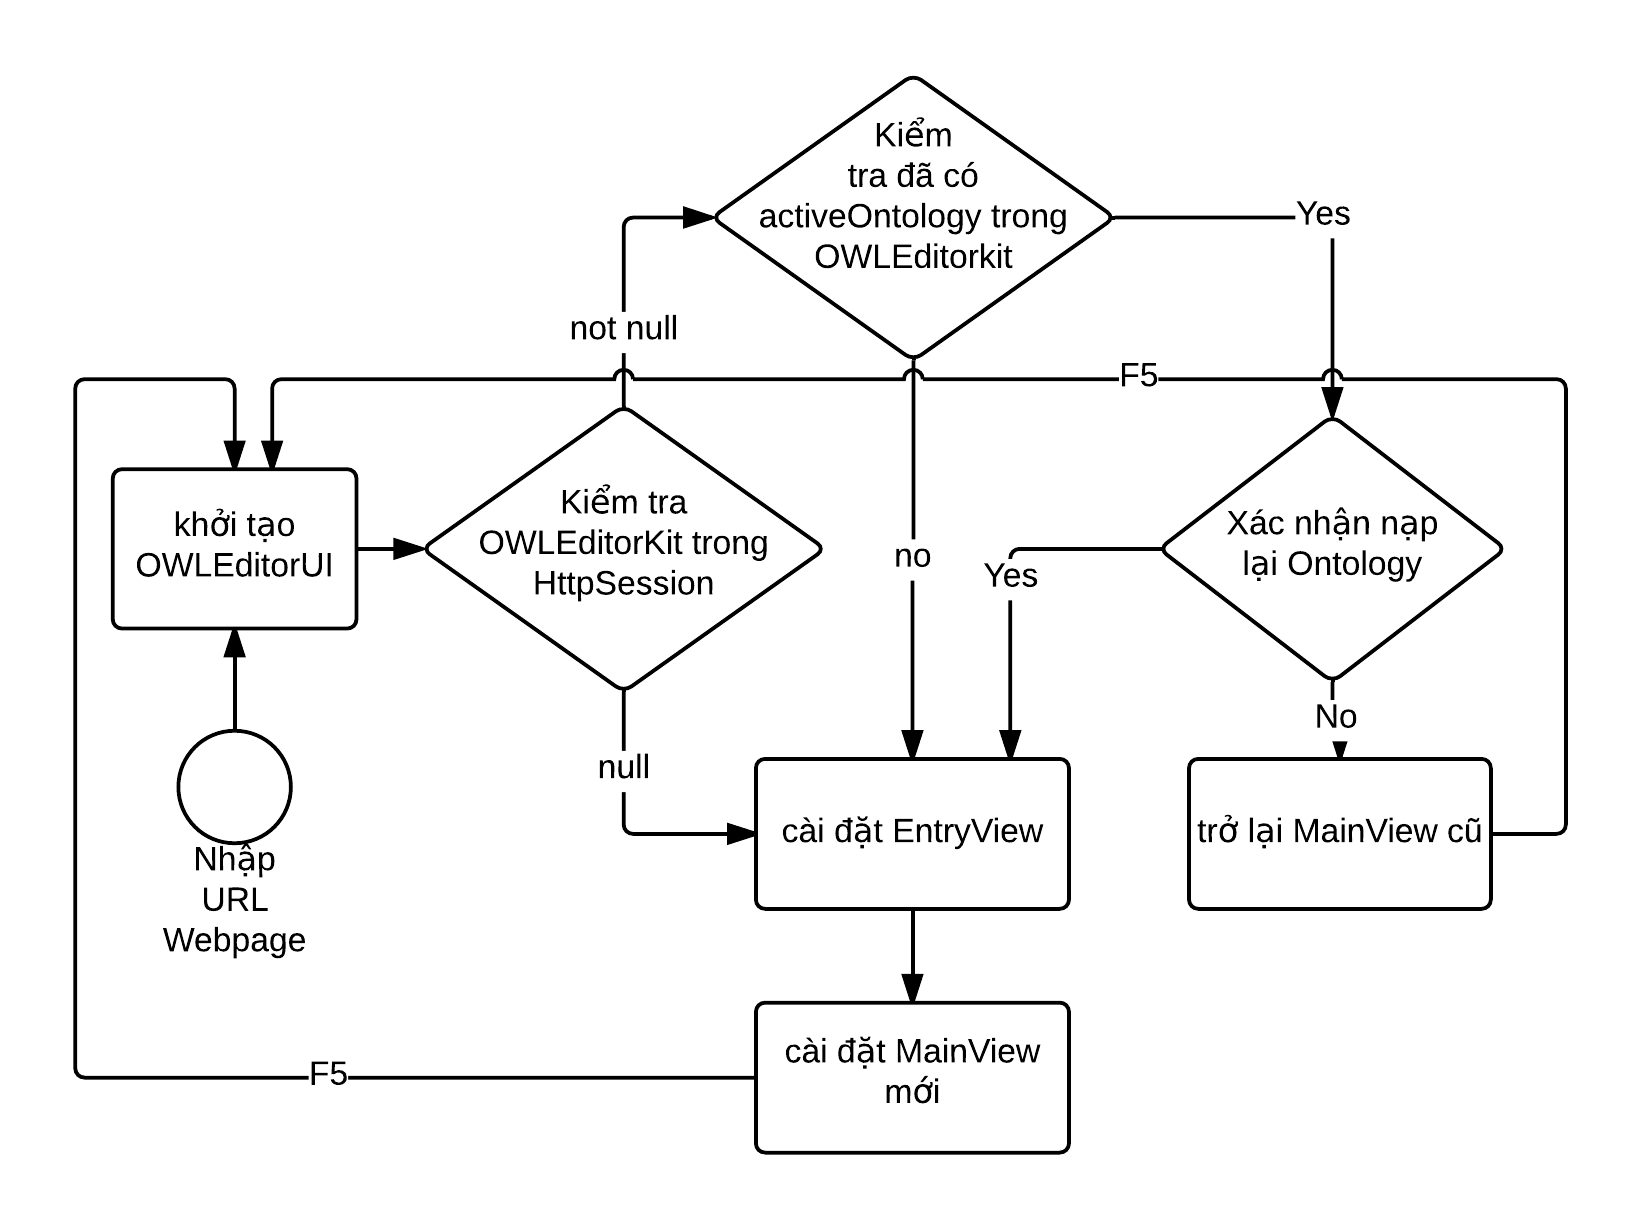
\includegraphics[width=150mm]{Figures/owleditorui_flowchart.png}
	\caption{Vòng đời của các view trong OWLEditorUI \label{overflow}}
\end{figure}
Mỗi lần chúng ta vào trang url của ứng dụng hay refresh thì vòng đời của các View sẽ diễn ra như trong hình 4.1. Việc kiểm tra các điều kiện đều nằm trong phương thức \textbf{updateContent} của OWLEditorUI.
\textbf{Tóm lại} OWLEditorUI là nơi sẽ cung cấp các thành phần lõi của hệ thống như OWLEditorKit, EventBus và HttpSession. Tiếp theo, chúng em sẽ trình bày cách xây dựng các View và thành phần của chúng.
\section{Xây dựng EntryView}
Như được thiết kế thì giao diện của EntryView tương đối đơn giản, chỉ có 1 panel chứa các input để nạp ontology theo 3 tùy chọn:
\begin{enumerate}
\item Nạp ontology qua URL. URL này bắt buộc phải là một tài liệu được định dạng theo tiêu chuẩn OWL 2 (RDF/XML, OWL/XML, FunctionalSyntax/XML,...).
\item Upload một tập tin chứa tài liệu Ontology và nạp tài liệu ontology này vào.
\item Tạo mới một tài liệu ontology.
\end{enumerate}
{\let\thefootnote\relax\footnotetext{
	\begin{enumerate}
		\item \textit{HorizontalLayout} các UI Component được sắp xếp theo chiều ngang, từ trái qua phải.
		\item \textit{VerticalLayout} các UI Component được sắp xếp theo chiều dọc, từ trên xuống.
		\item \textit{AbsoluteLayout} các UI Component được sắp xếp theo đúng vị trí tọa độ được khai báo.
		\item \textit{CssLayout} các UI Component được sắp xếp theo định nghĩa từ các file css tương ứng.
	\end{enumerate}}
}
\begin{figure}[h!]
	\centering
	\frame{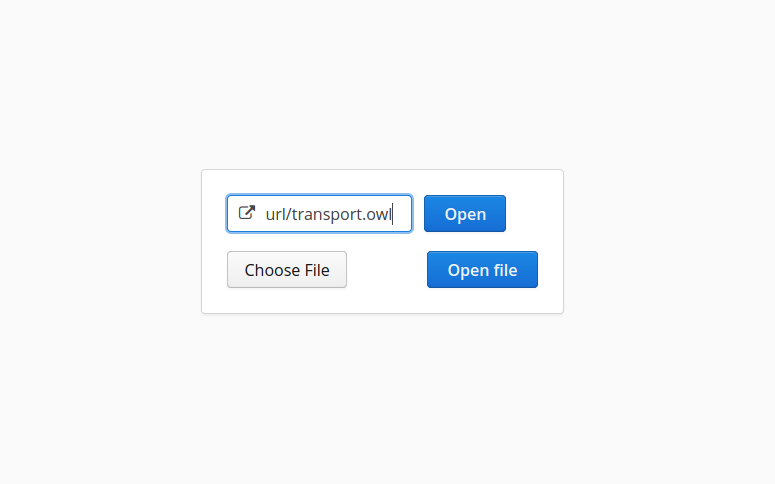
\includegraphics[width=145mm]{Figures/owleditor_entryview.png}}
	\caption{EntryView đã xây dựng\label{overflow}}
\end{figure}
Giao diện EntryView được mở rộng từ layout \textit{VerticalLayout}\textsuperscript{*}, để chứa panel ở giữa - panel này cũng là một \textit{VerticalLayout} tập hợp mỗi dòng là một \textit{HorizontalLayout}, mỗi \textit{HorizontalLayout} này sẽ chứa một \textit{TextField} và một \textit{Button} hoặc một \textit{UploadField} và một \textit{Button} (Hình 4.2) - tất cả các thành phần vừa nêu đều được cung cấp bởi Vaadin. Nhờ vậy, việc xây dựng giao diện khá dễ dàng, chẳng hạn để đặt vị trí trung tâm cho panel trong hình chỉ cần 
\begin{verbatim}
setComponentAlignment(entriesPanel, Alignment.MIDDLE_CENTER);
\end{verbatim}
Sau khi click "Open", nếu URL chứa tài liệu hợp lệ thì nó sẽ được nạp vào trong OWLEditorKit, nếu đây là lần đầu OWLEditorKit được sử dụng và chưa được lưu trong HttpSession thì lưu nó vào Session và cuối cùng là chuyển giao diện qua \textit{MainView} (Hình 4.1). Quá trình tương tự cũng xảy ra khi nạp tài liệu từ tập tin upload và tạo mới tài liệu, riêng việc tạo tài liệu thì chúng ta có thể tùy chọn đặt 1 IRI cho nó trong TextField ở dòng cuối. Upload file cũng là một plugin được cung cấp qua \cite{vaadindirectory} việc sử dụng cũng rất đơn giản.
\begin{verbatim}
UploadField uf = new UploadField();
// code bên trong "Open" Button ClickListener
File file = (File) uf.getValue();
OWLEditorUI.getEditorKit() // Nạp ontology vào trong OWLEditorKit
           .loadOntologyFromOntologyDocument(IRI.create(file));
OWLEditorUI.getHttpSession() // lưu OWLEditorKit trong Session
           .setAttribute("OWLEditorKit", OWLEditorUI.getEditorKit());
// Đặt giao diện là MainView 
UI.getCurrent().setContent(new MainView());                    
\end{verbatim}

\section{Xây dựng MainView}
Trong thiết kế \textit{MainView} sẽ là nơi chứa tất cả các Tab của ứng dụng, các tab này được xây dựng dựa trên thành phần \textit{TabSheet} của Vaadin, mỗi tab đều có thể là bất cứ thành phần giao diện nào của Vaadin (UIComponent và Layout của Vaadin đều có chung Interface \textit{Component}). Do vậy, nội dung của MainView khá đơn giản:
\begin{verbatim}
public class MainView extends HorizontalLayout {
  final TabSheet root = new TabSheet();
  public MainView() {
    root.addTab(new ClassesSheet(), "Classes");
    addComponent(root); // Thêm TabSheet vào layout của MainView;
    ...}
} 
\end{verbatim}
\subsection{Xây dựng Tab dùng mô tả lớp, thuộc tính đối tượng/dữ liệu và cá thể}
Do bố cục phần lần các thành phần trong các Tab này cũng tương đối giống nhau, nên chúng em chỉ xin lấy Tab Class (lớp) ra trình bày chi tiết, còn những tab còn lại chúng em chỉ xin trình bày những thành phần khác của chúng so với Tab Class.
\subsubsection{ClassSheet}
Đây là lớp chúng em dùng để tổ chức các thành phần giao diện dành để tương tác với các lớp trong OWL 2 Ontology.
\begin{figure}[h!]
	\centering
	\frame{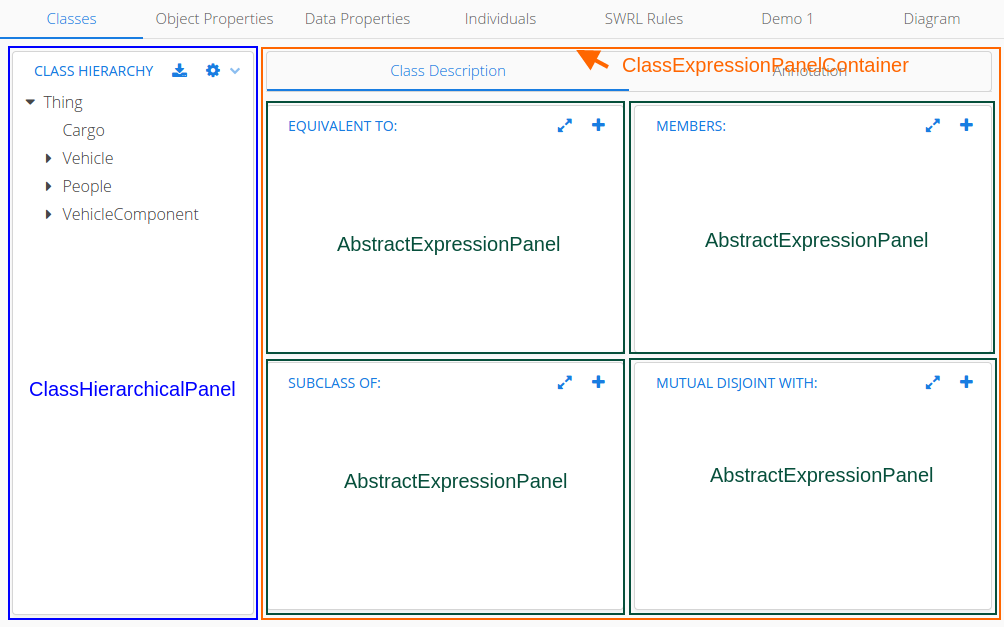
\includegraphics[width=155mm]{Figures/owleditor_mainview.png}}
	\caption{ClassSheet(Tab dành cho lớp) đã xây dựng\label{overflow}}
\end{figure}
{\let\thefootnote\relax\footnotetext{
		Lưu ý:  \textit{ClassHierarchicalPanel}, \textit{ObjectPropertyHierachicalPanel} và \textit{DataPropertyHierarchicalPanel} đều kế thừa từ \textit{AbstractHierarchyPanel}.
}}
Ở bên trái là một Panel gọi là \textit{ClassHierarchicalPanel} mở rộng từ \textit{AbstractHierarchyPanel} \textsuperscript{*} được chúng em xây dựng với mục tiêu là biểu diễn các lớp trong OWL 2 Ontology, và cho phép thực hiện các thao tác thêm lớp con, lớp cùng họ (sibling) và xóa lớp bằng cách click phải vào bất kì node nào trên cây. Ở góc phải bên trên của panel này, với kí hiệu bánh răng với chức năng thêm xóa tương tự, ngoài ra còn có tính năng bật reasoner cho hệ thống. Kế bên kí hiệu bánh răng, là một kí hiệu tải xuống, khi click sẽ lưu lại trạng thái ontology hiện hành và tải xuống dưới định dạng OWL/XML.
\\
Bên trong \textit{ClassHierarchicalPanel} có thành phần \textit{Tree} đây chính là thành phần sẽ liên kết với dữ liệu từ các \textit{HiearchicalContainer} được giới thiệu trong mục tổ chức dữ liệu ở chương trước, ở đây cụ thể nó sẽ liên kết với các \textit{ClassHierarchicalContainer} - chứa các lớp trong ontology với cấu trúc phân cấp. Nếu đúng như trong thiết kế thì chúng em sẽ sử dụng EventBus để xử lý các sự kiện thêm/xóa lớp ở đây, tuy nhiên sau khi xây dựng xong chúng em gặp phải vấn đề về con-current event - nghĩa khi thực hiện thao tác thêm/xóa sẽ có 2 event giống nhau được tạo ra và truyền lên EventBus. Do vẫn chưa tìm được nguyên nhân chính xác, nên chúng em đã qua về với thiết kế truyền thống của Java là tạo một interface \textit{OWLEntityActionHandler} vào áp dụng nó vào thành phần \textit{Tree}. Thiết kế này yêu cầu các đối tượng giao tiếp các sự kiện với nhau phải biết nhau.
\begin{figure}[h!]
	\centering
	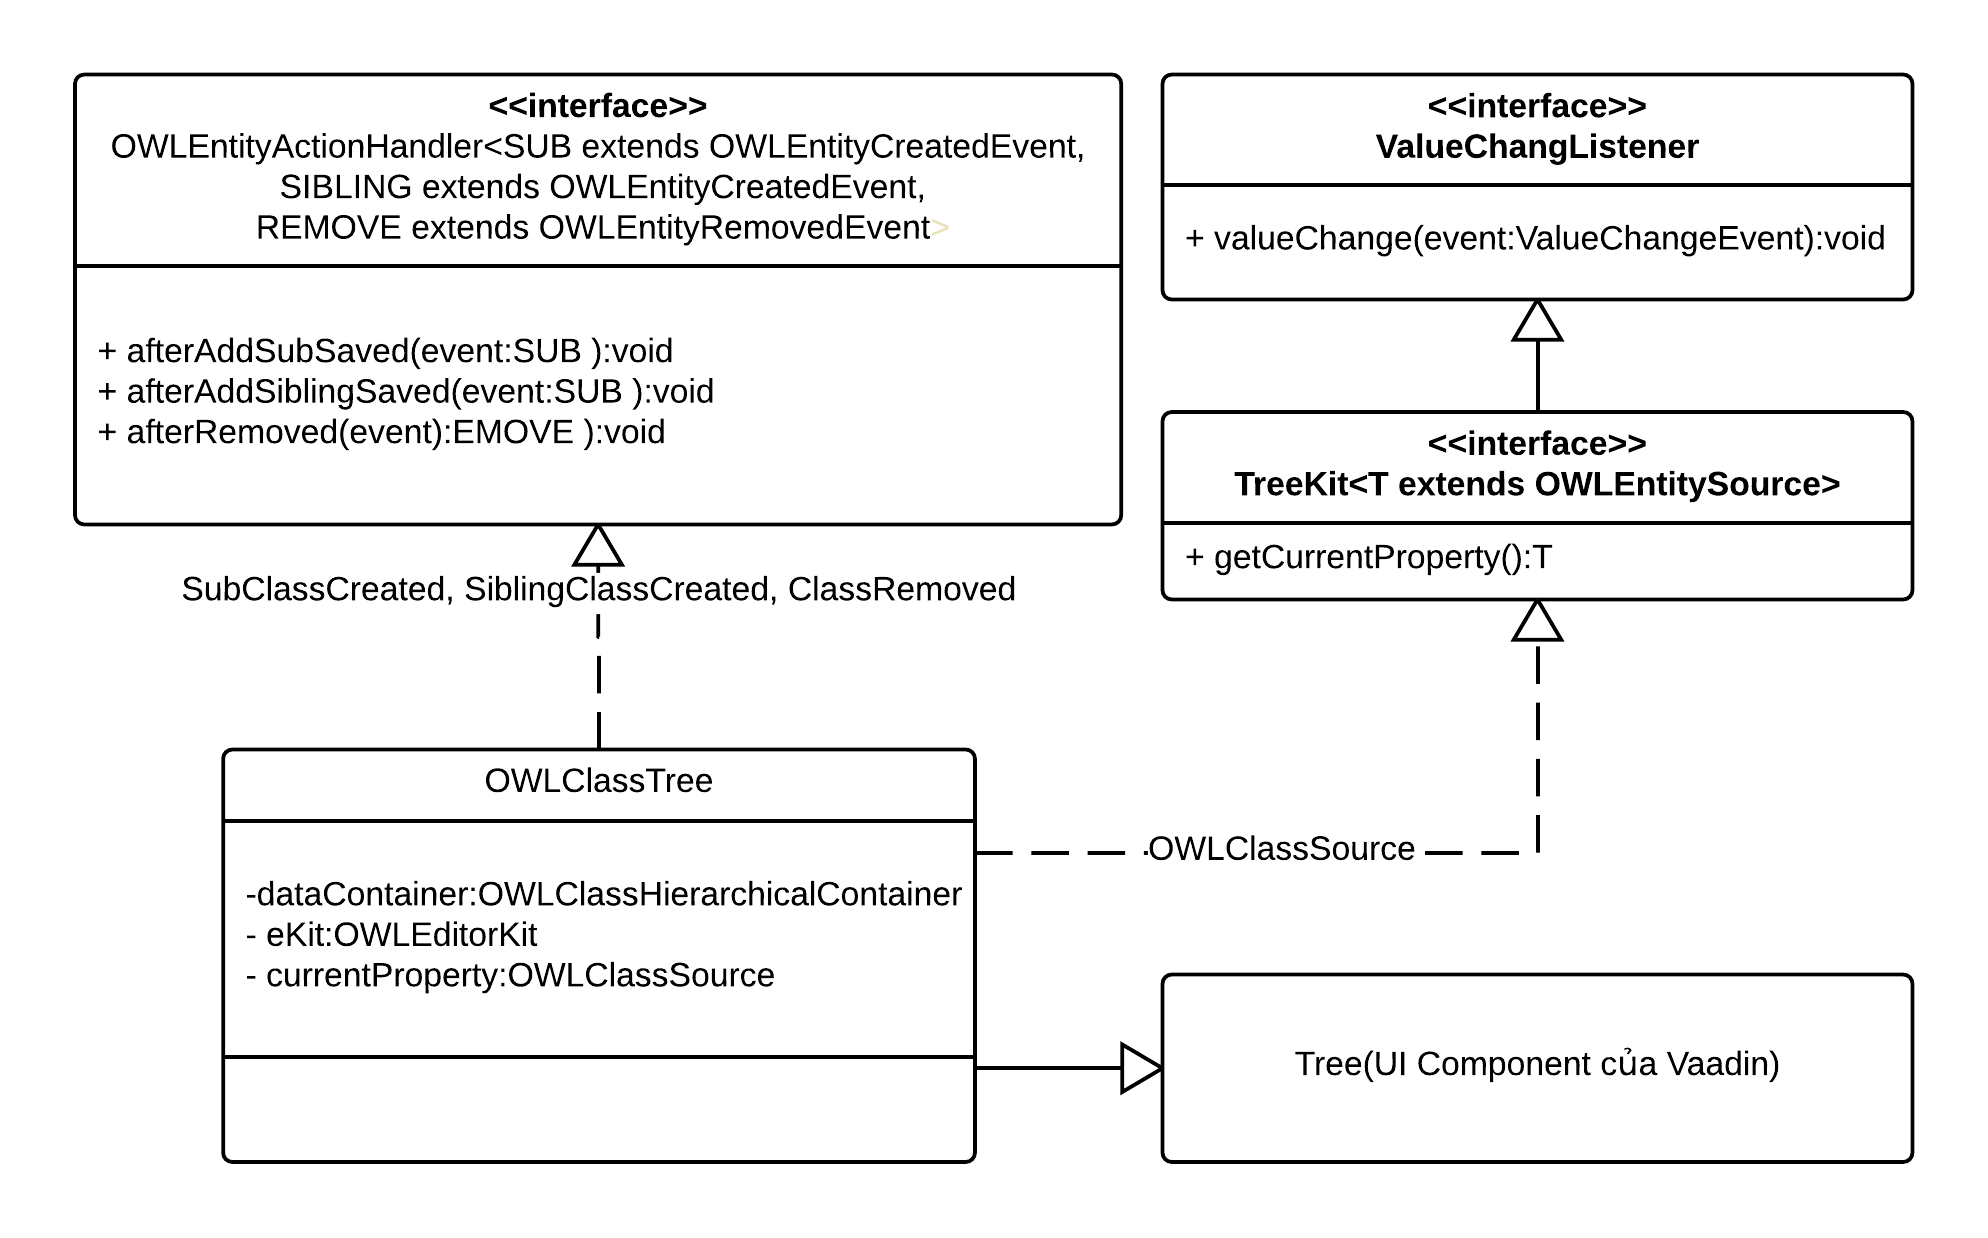
\includegraphics[width=155mm]{Figures/uml_owlclasstree.png}
	\caption{Cây OWLClassTree hiển thi các lớp trong Ontology trong ClassSheet \label{overflow}}
\end{figure}

